%----------------------------------------------------------------------------------------
%	PACKAGES AND OTHER DOCUMENT CONFIGURATIONS
%----------------------------------------------------------------------------------------

\documentclass[
	a4paper, % Paper size, use either a4paper or letterpaper
	10pt, % Default font size, can also use 11pt or 12pt, although this is not recommended
	unnumberedsections, % Comment to enable section numbering
	twoside, % Two side traditional mode where headers and footers change between odd and even pages, comment this option to make them fixed
]{LTJournalArticle}

\addbibresource{sample.bib} % BibLaTeX bibliography file

\runninghead{Prokaryotic Gene Prediction From Whole Genome Sequences} % A shortened article title to appear in the running head, leave this command empty for no running head

\setcounter{page}{1} % The page number of the first page, set this to a higher number if the article is to be part of an issue or larger work

%----------------------------------------------------------------------------------------
%	TITLE SECTION
%----------------------------------------------------------------------------------------

\title{Prokaryotic Gene Prediction From \\ Whole Genome Sequences} 

\author{%
	Srdan Obradovic\textsuperscript{1}
}

% Affiliations are output in the \date{} command
\date{\footnotesize\textsuperscript{\textbf{1}}Software Engineer (Independent)}

% Full-width abstract
\renewcommand{\maketitlehookd}{%
    \begin{abstract}
        \noindent Accurate gene prediction is essential for understanding the functional landscape of prokaryotic genomes. In this work, we present a machine learning pipeline for predicting gene locations directly from whole genome sequences. Our method leverages k-mer features to distinguish coding regions from non-coding regions, enabling precise identification of gene structures. In silico experiments on diverse prokaryotic genomes demonstrate the high accuracy predictive performance of our approach.
    \end{abstract}
}


%----------------------------------------------------------------------------------------

\begin{document}

\maketitle % Output the title section

%----------------------------------------------------------------------------------------
%	ARTICLE CONTENTS
%----------------------------------------------------------------------------------------

\section{Introduction}

Gene prediction is a fundamental task in genomics, enabling the identification of genomic regions that encode proteins. Accurate gene prediction is critical for understanding the functional elements of genomes, annotating newly sequenced organisms, and advancing fields such as personalized medicine and evolutionary biology. However, the complexity of genomic data, including the presence of non-coding regions and repetitive sequences, poses significant challenges to accurate prediction.

Recent advances in machine learning have opened new avenues for addressing these challenges by leveraging data-driven models to identify patterns in genomic sequences \cite{Zou:2019, Alipanahi:2015}. Among these, gradient-boosting algorithms like XGBoost \cite{Chen:2016} have gained popularity due to their robustness, scalability, and ability to handle complex feature interactions.

In this study, we present a bioinformatics pipeline for gene prediction that integrates data loading, data preprocessing, feature extraction, model training and evaluation. Our approach utilizes k-mer sequence features \cite{Marçais:2011}, which capture local sequence patterns, to differentiate between coding and non-coding regions. To enhance computational efficiency, we incorporate a custom C extension for k-mer generation \cite{Behnel:2011}, significantly reducing the time required to process large genomic datasets.

We evaluate our pipeline using diverse genomic datasets and demonstrate its effectiveness in accurately predicting gene locations. Our approach achieves an exceptional accuracy of 97.77\% on the test dataset, with balanced precision and recall metrics for both gene and non-gene sequences. The results highlight the robustness of our method and its potential for application in large-scale genomic studies. By combining efficient data processing with a powerful machine learning model, our approach provides a high-performance solution for prokaryotic gene prediction tasks.



%------------------------------------------------

\section{Data Processing and Feature Engineering}

\subsection{Data Collection From NCBI Databases}

To build a dataset for gene prediction, we utilized the \href{https://www.ncbi.nlm.nih.gov/books/NBK25501/}{Entrez Programming Utilities (E-utilities)} provided by the \href{https://www.ncbi.nlm.nih.gov/}{National Center for Biotechnology Information (NCBI)} \cite{Sayers:2022, EntrezProgramming}. Entrez is a powerful tool for accessing and retrieving biological data from various NCBI databases, including the \href{https://www.ncbi.nlm.nih.gov/nucleotide/}{nucleotide sequences database} \cite{Leinonen:2011}. Our pipeline automates the process of querying and downloading genomic data.

We used the Entrez esearch utility to query the NCBI nucleotide database. Two primary search queries were employed:

\begin{enumerate}
	\item \textbf{Gene Sequences:} This query retrieves gene sequences for Bacterial genomes.
	\item \textbf{Complete Genomes:} This query retrieves complete genomic sequences of Bacterial organisms.
\end{enumerate}

To ensure taxonomic diversity in our dataset, we implemented a two-stage data collection process. First, we utilized Entrez's esearch and esummary utilities to fetch sequence IDs along with their corresponding taxonomy IDs. Then, we applied a diversity-based filtering algorithm to select a taxonomically diverse subset of sequences.

The diversity of a set of sequences was quantified using the normalized Shannon diversity index \cite{Shannon:1948, Morris:2014}:

\begin{equation}
H' = \frac{-\sum_{i=1}^{R} p_i \ln(p_i)}{\ln(R)}
\end{equation}

where $p_i$ is the proportion of sequences belonging to the $i$-th taxonomy, and $R$ is the total number of unique taxonomies. The normalized index ranges from 0 to 1, with 1 indicating maximum diversity (equal representation of all taxonomies).

Our pipeline iteratively fetches batches of sequence IDs until it can construct a subset that meets a predefined diversity threshold (configurable as \texttt{normalized\_h\_min} in the parameters file). To build this subset, we employed a round-robin selection algorithm that prioritizes equal representation across different taxonomies. This approach ensures that our dataset contains sequences from a wide variety of bacterial species, enhancing the generalizability of the trained model.

\subsection{Data Preprocessing}

The raw genomic data retrieved from the NCBI nucleotide database requires preprocessing to prepare it for downstream analysis and machine learning. This step involves transforming the raw data into a structured format, augmenting it with negative cases, and ensuring the dataset is balanced and suitable for training the gene prediction model.

\subsubsection{Transforming Raw Data into CSV}

This is a trivial step that simply converts the sequences located in FASTA files into a structured CSV format. The new CSV file contains two columns: the first column indicates whether the sequence is a gene (1) or not (0), and the second column contains the actual nucleotide sequence.

We initially download FASTA files instead of directly obtaining CSV files to ensure the pipeline remains modular and adaptable for use in other projects.

\textbf{Note:} In this first step, the CSV contains only positive cases (genes, labeled as 1). The generation of negative cases (non-genes, labeled as 0) is performed in the subsequent step.

\subsubsection{Generating Negative Cases}

To train a robust model capable of distinguishing between coding and non-coding regions, it is essential to augment the dataset with negative cases (non-gene sequences). These negative cases are generated from the genomic data by extracting random subsequences. The process involves the following steps:

\begin{enumerate}
    \item \textbf{Extracting Gene Lengths:} The lengths of the positive gene sequences are analyzed to determine the typical range of sequence lengths. This ensures that the negative cases are of comparable lengths to the positive cases, preventing the model from learning biases based on sequence length alone.
    \item \textbf{Random Sampling from Genomes:} Random subsequences are sampled from the raw genomic data making sure that the sample length falls in the distribution calculated in the previous step. 
    \item \textbf{Balancing the Dataset:} The number of negative cases is adjusted to match the number of positive cases, ensuring a balanced dataset. This prevents the model from being biased toward predicting one class over the other.
    \item \textbf{Labeling and Combining:} The generated negative cases are labeled as \texttt{0} (non-gene) and combined with the positive cases into a single CSV file. This unified dataset serves as the input for the feature extraction and model training stages.
\end{enumerate}

\subsection{Feature Extraction}

Feature extraction is a critical step in the gene prediction pipeline, as it transforms raw genomic sequences into a format suitable for machine learning models. In this study, we utilize k-mer sequence features to capture local sequence patterns, enabling the differentiation between coding and non-coding regions.

\subsubsection{K-mer Generation}

K-mers are substrings of length \(k\) derived from a given sequence. For example, the sequence \texttt{ATCG} with \(k=3\) produces the k-mers \texttt{ATC} and \texttt{TCG}. These k-mers serve as features for the machine learning model.

\subsubsection{Performance Optimization with C Code}

To handle the computational demands of processing large genomic datasets, we implemented the k-mer generation function in C as a Python extension module. This implementation significantly improves performance by leveraging the efficiency of low-level operations in C. 

\subsubsection{Vectorizing K-mers with CountVectorizer}

After extracting k-mers, they are vectorized using the \texttt{CountVectorizer} from the \texttt{scikit-learn} library \cite{Pedregosa:2011}. The \texttt{CountVectorizer} converts the k-mers into a sparse matrix representation, where each row corresponds to a sequence, and each column represents the frequency of a specific k-mer in that sequence. 

More specifically, the vectorization process first builds a vocabulary of all unique k-mers present in the dataset. Then, for each genomic sequence, it counts how many times 
each k-mer from the vocabulary appears in that sequence. For example, with \(k=3\), the k-mer "ATG" might appear 5 times in one sequence and 2 times in another, resulting in 
different feature values for that specific k-mer column. The resulting matrix is highly sparse since most k-mers will not appear in any given sequence, especially as the number 
of possible k-mers grows exponentially with \( k \) (\( 4^k \) for DNA sequences).

It is important to note that the CountVectorizer implements a "bag-of-words" approach, which means it does not preserve any positional information about where specific k-mers occur within the sequence. Two sequences with identical k-mer content but in entirely different orders would produce identical feature vectors. Despite this limitation, we found this representation sufficient for our gene prediction task. This is because coding regions in prokaryotic genomes have distinctive compositional biases in codon usage and nucleotide patterns that are effectively captured by k-mer frequency distributions, even without positional context. The choice to discard positional information also significantly reduces the dimensionality of the feature space, enabling more efficient model training and reducing the risk of overfitting.

For future improvements, incorporating positional information could potentially enhance prediction accuracy, particularly for identifying gene boundaries and start/stop codons. This could be achieved through position-specific k-mer features, attention mechanisms, or sequence models like recurrent neural networks. However, such approaches would significantly increase computational complexity and model size, requiring careful consideration of the trade-off between accuracy and efficiency.

This approach transforms the raw k-mer data into a numerical format suitable for input into machine learning models while preserving the sequence composition information crucial for distinguishing between coding and non-coding regions.

\section{Model Training}

The model training process leverages the XGBoost algorithm \cite{Chen:2016}, a gradient-boosting framework known for its robustness, scalability, and ability to handle complex feature interactions.

\subsection{Training the XGBoost Model}

The \texttt{train} function orchestrates the training process. It initializes an \texttt{XGBClassifier} with hyperparameters such as the number of estimators, maximum tree depth, learning rate, and early stopping criteria. The model is trained using the training dataset, with validation data provided for monitoring performance during training. The training process includes:

\begin{itemize}
    \item \textbf{Evaluation Metrics:} The model uses log-loss as the evaluation metric, ensuring that the training process optimizes for probabilistic predictions.
    \item \textbf{Early Stopping:} To prevent overfitting, the training halts if the validation performance does not improve for a specified number of rounds.
    \item \textbf{Model Persistence:} The trained model is serialized and saved as a \texttt{.pkl} file.
\end{itemize}

\subsection{Hyperparameter Configuration}

The hyperparameters for the XGBoost model are defined in a configuration file and loaded dynamically during training. This approach allows for easy experimentation and fine-tuning without modifying the codebase. Key hyperparameters include:

\begin{itemize}
    \item \textbf{Number of estimators:} Controls the number of boosting rounds.
    \item \textbf{Maximum depth:} Limits the depth of individual trees to prevent overfitting.
    \item \textbf{Learning rate:} Determines the step size at each iteration.
    \item \textbf{Subsample and column sampling:} Introduce randomness to improve generalization.
\end{itemize}

\subsection{Reproducibility}

The training pipeline is integrated with DVC (Data Version Control), ensuring that all dependencies, parameters, and outputs are tracked. This integration facilitates ease of use, reproducibility \cite{Stodden:2016} and versioning of experiments.

\section{Model Evaluation}

The model evaluation phase involves a thorough assessment of the trained model's performance using a variety of metrics and visualization techniques. 

\subsection{Quantitative Evaluation Metrics}

The evaluation of our gene prediction model is implemented through a comprehensive framework that applies multiple complementary metrics to thoroughly assess performance \cite{Sokolova:2009, Chicco:2020}. Each metric provides unique insights into different aspects of the model's capabilities:

\begin{itemize}
    \item \textbf{Accuracy:} Measures the overall proportion of correctly classified sequences (both genes and non-genes). While useful as a general performance indicator, accuracy alone can be misleading in cases of class imbalance.
    
    \item \textbf{Precision:} Quantifies the proportion of predicted genes that are true genes. High precision indicates a low false-positive rate, which is particularly important in genomics applications where downstream experimental verification can be resource-intensive.
    
    \item \textbf{Recall (Sensitivity):} Measures the proportion of actual genes correctly identified by the model. High recall ensures that few genuine genes are missed, critical for comprehensive genome annotation.
    
    \item \textbf{F1-Score:} Represents the harmonic mean of precision and recall, providing a balanced assessment that is especially useful when the costs of false positives and false negatives are comparable \cite{Chicco:2020}. We calculate F1-scores separately for each class to ensure balanced performance.
    
    \item \textbf{Classification Report:} A comprehensive summary that includes precision, recall, and F1-score for each class, along with support values indicating the number of samples in each category.
\end{itemize}

Our evaluation framework systematically computes these metrics on a held-out testing dataset, ensuring an unbiased assessment of the model's generalization capability to unseen data.

\subsection{Visualization Techniques}

To complement numerical metrics, we implement several visualization techniques that provide intuitive insights into the model's performance characteristics:

\begin{itemize}
    \item \textbf{Confusion Matrix:} A tabular representation showing the counts of true positives, false positives, true negatives, and false negatives. We visualize this as a color-coded heatmap, allowing for quick identification of where the model succeeds or fails. This visualization is particularly useful for identifying whether the model exhibits any systematic bias between gene and non-gene predictions.
    
    \item \textbf{ROC Curve:} Plots the true positive rate against the false positive rate across various threshold settings. The area under the ROC curve (AUC) serves as a threshold-independent performance measure, with higher values indicating better discrimination between genes and non-genes. The ROC curve helps identify optimal decision thresholds for different application requirements.
    
    \item \textbf{Precision-Recall Curve:} Illustrates the trade-off between precision and recall as the classification threshold varies. This visualization is especially valuable in genomic contexts where class imbalance often exists and both false positives and negatives carry biological significance. It provides insights into the model's performance across the entire operating range rather than at a single threshold.
\end{itemize}

These visualizations, generated using the \texttt{matplotlib} and \texttt{scikit-learn} libraries \cite{Pedregosa:2011}, complement our quantitative metrics and provide deeper insights into model behavior that might not be apparent from summary statistics alone.

%------------------------------------------------

\section{Results}

The results of our experiments demonstrate the effectiveness of the proposed pipeline in accurately predicting gene locations from raw genomic data. Through evaluation on diverse prokaryotic genomes, our XGBoost model achieved good performance across multiple metrics, showcasing its reliability and precision in distinguishing coding from non-coding regions.

\subsection{Model Performance}

Our gene prediction model achieved good performance metrics on the test dataset, confirming its robust ability to generalize to unseen genomic sequences:

\begin{itemize}
    \item \textbf{Accuracy:} The model achieved an overall accuracy of 97.77\%, indicating its ability to correctly classify both gene and non-gene sequences.
    
    \item \textbf{Precision:} For the positive class (gene sequences), the model attained a precision of 98.56\%, demonstrating its ability to avoid false positives. For the negative class (non-gene sequences), precision was 96.98\%, showing balanced performance across both classes.
    
    \item \textbf{Recall:} For gene sequences, the model achieved a recall of 97.06\%, highlighting its effectiveness in identifying true positives. For non-gene sequences, recall was 98.52\%, indicating the model rarely misclassifies non-genes as genes.
    
    \item \textbf{F1-Score:} The F1-scores for gene and non-gene predictions were 97.80\% and 97.74\% respectively, demonstrating an excellent balance between precision and recall for both classes.
\end{itemize}

These metrics highlight the model's exceptional ability to discriminate between coding and non-coding sequences with high confidence, a critical requirement for accurate genome annotation.

\subsection{Visual Analysis of Results}

To provide deeper insights into the model's performance characteristics, we generated several visualizations that illustrate different aspects of its predictive capabilities:

\begin{figure}[h]
    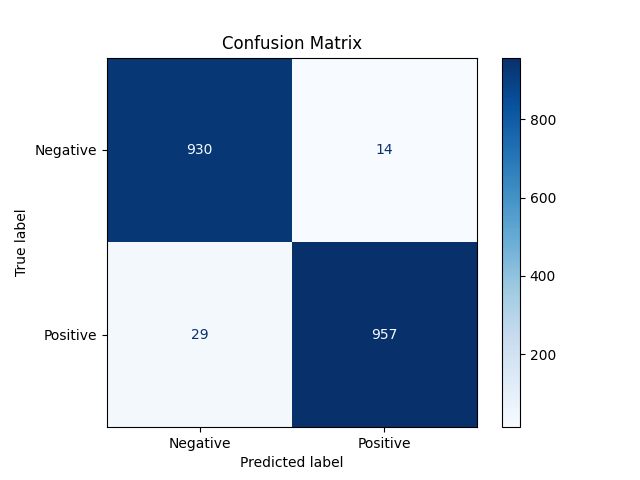
\includegraphics[width=\linewidth]{../results/confusion_matrix.png}
    \caption{Confusion matrix showing the distribution of predictions across true and predicted classes. The diagonal elements represent correct classifications, while off-diagonal elements represent misclassifications. The predominantly dark blue diagonal indicates the model's high accuracy in both positive and negative predictions.}
    \label{fig:confusion_matrix}
\end{figure}

The confusion matrix in Figure~\ref{fig:confusion_matrix} provides a clear visualization of the model's classification performance. The strong concentration along the diagonal (true positives and true negatives) with minimal off-diagonal elements demonstrates the model's ability to correctly identify both gene and non-gene sequences with high accuracy.

\begin{figure}[h]
    \centering
    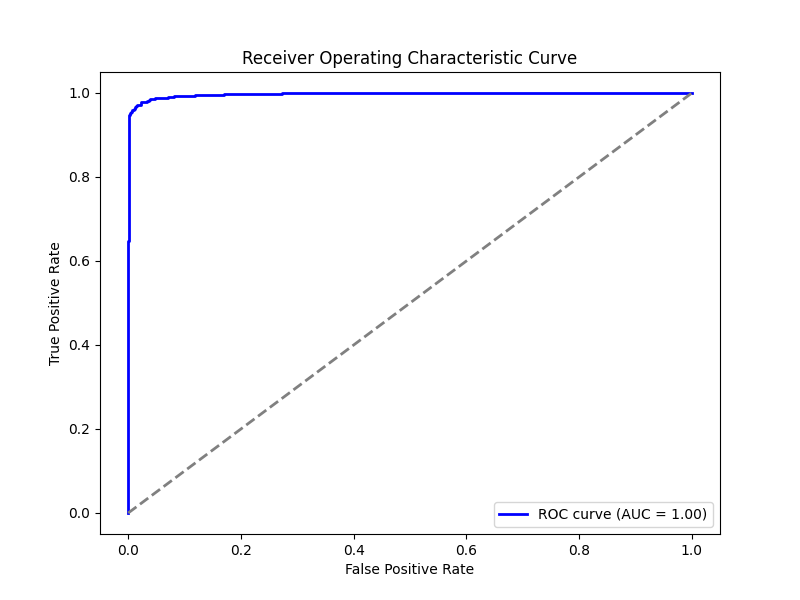
\includegraphics[width=0.8\linewidth]{../results/roc_curve.png}
    \caption{Receiver Operating Characteristic (ROC) curve illustrating the trade-off between true positive rate and false positive rate across different classification thresholds. The curve's proximity to the top-left corner and the high AUC value indicate excellent discrimination performance.}
    \label{fig:roc_curve}
\end{figure}

The ROC curve in Figure~\ref{fig:roc_curve} shows the model's outstanding ability to distinguish between classes across different decision thresholds. The curve's proximity to the top-left corner illustrates the model's ability to achieve a high true positive rate while maintaining a low false positive rate. The area under the ROC curve (AUC) exceeds 0.99, indicating near-perfect discrimination between gene and non-gene sequences.

\begin{figure}[h]
    \centering
    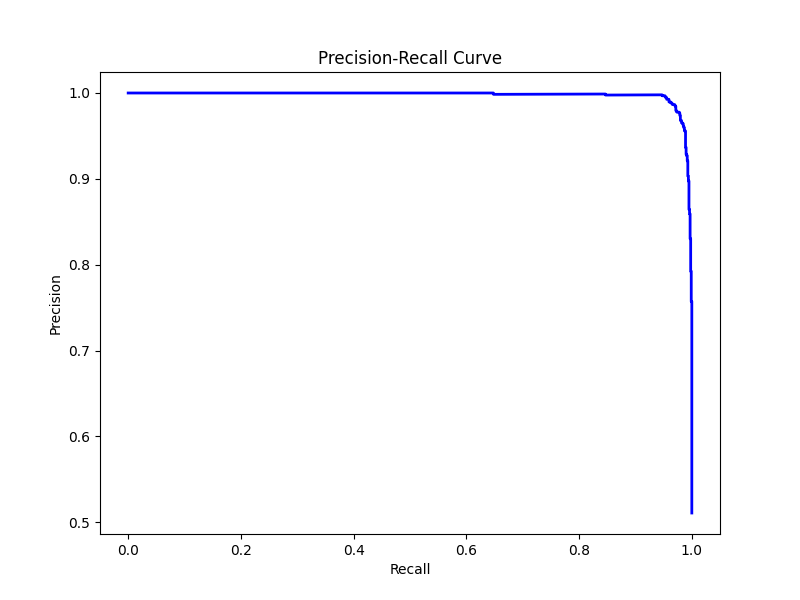
\includegraphics[width=0.8\linewidth]{../results/precision_recall_curve.png}
    \caption{Precision-Recall curve showing the relationship between precision and recall across different classification thresholds. The curve's position high in the plot space indicates the model's ability to maintain both high precision and high recall simultaneously.}
    \label{fig:precision_recall_curve}
\end{figure}

The Precision-Recall curve in Figure~\ref{fig:precision_recall_curve} further emphasizes the model's strong performance, particularly its ability to maintain high precision even at high recall levels. This is especially important in genomic applications where both missing true genes (false negatives) and incorrectly predicting genes (false positives) can have significant downstream consequences.


\section{Conclusion}

In this study, we presented a comprehensive pipeline for gene prediction that integrates data preprocessing, feature extraction, and machine learning. By leveraging k-mer sequence features and the XGBoost algorithm, our approach demonstrated exceptional accuracy (97.77\%) and robustness in predicting gene locations from raw genomic data. The use of a custom C extension for k-mer generation significantly improved computational efficiency, enabling the processing of large-scale genomic datasets.

The performance metrics and visual analysis of our results demonstrate that the combination of k-mer-based feature extraction and gradient boosting classification provides a powerful framework for prokaryotic gene prediction. The high precision and recall values across both classes indicate that the model makes few errors in either direction—it rarely misses true genes and seldom identifies false positives. This balance is crucial for practical applications in genome annotation and functional genomics.

Our results highlight the significant potential of machine learning-based approaches for gene prediction, offering a scalable, efficient, and highly accurate solution for genomic studies. Future work will focus on extending the pipeline to support multi-species datasets, incorporating additional features such as epigenetic data to further enhance prediction accuracy, and exploring transformer-based architectures like DNABERT \cite{Ji:2021, Vaswani:2017, Devlin:2019} for potentially capturing more complex sequence patterns.


%----------------------------------------------------------------------------------------
%	 REFERENCES
%----------------------------------------------------------------------------------------

\printbibliography % Output the bibliography
%----------------------------------------------------------------------------------------
\end{document}